\documentclass[a4paper,1pt]{article}
\usepackage[utf8]{inputenc}
\usepackage[main=english]{babel}
\usepackage[rightcaption]{sidecap}
% \usepackage{minted}
\usepackage{graphicx}
\usepackage[colorlinks=true, allcolors=red]{hyperref}
\usepackage{sectsty}
\usepackage[paperheight=29.7cm,paperwidth=21cm,textwidth=15cm]{geometry} %A4 size
\usepackage{fancyhdr}
\usepackage[siunitx]{circuitikz}
\usepackage{tabularx}
\usepackage{physunits}
\usepackage{booktabs}
\usepackage{tikz}
\usepackage{pgfplots}
\usepackage{karnaugh-map}
\usepackage[nocompress]{cite}
\usepackage{cite}
\usepackage{parskip}
\usepackage{amsmath,amssymb,amsfonts}
\usepackage{algorithmic}
\usepackage{listings}
\usepackage{xcolor}
% The preceding line is only needed to identify funding in the first footnote. If that is unneeded, please comment it out.
\usepackage{textcomp}
 % More defined colors
% We will externalize the figures
\usepackage{fancyvrb}
\usepackage{struktex}
\usepackage{marginnote}
\usepackage{float} 
\renewcommand*{\marginfont}{\color{blue}}

\definecolor{codegreen}{rgb}{0,0.6,0}
\definecolor{codegray}{rgb}{0.5,0.5,0.5}
\definecolor{codepurple}{rgb}{0.58,0,0.82}
\definecolor{backcolour}{rgb}{0.95,0.95,0.92}
% Footers/Headers opmaak:
\pagestyle{fancy}
\lhead{}
\chead{2223 1.4 BSc TI01: \textit{project netwerken}}
\rhead{}
\lfoot{\textit{Semih Can Karakoç}}
\cfoot{\textit{\today}}
\rfoot{\textit{\thepage}}
\renewcommand{\headrulewidth}{0.1pt}
\renewcommand{\footrulewidth}{0.4pt}

% Afbeelding settings:
\graphicspath{ {./Figures/} }
% \sectionfont{\left}
% \subsectionfont{\centering}
% \subsubsectionfont{\centering}

% Voorpagina opmaak:
\title{\textit{Project Netwerken}}
\author{{Semih Can Karakoç (695258)}}
\date{\textit{\today}}

\lstdefinestyle{mystyle}{
    backgroundcolor=\color{backcolour},   
    commentstyle=\color{codegreen},
    keywordstyle=\color{magenta},
    numberstyle=\tiny\color{codegray},
    stringstyle=\color{codepurple},
    basicstyle=\ttfamily\footnotesize,
    breakatwhitespace=false,         
    breaklines=true,                 
    captionpos=b,                    
    keepspaces=true,                 
    numbers=left,                    
    numbersep=5pt,                  
    showspaces=false,                
    showstringspaces=false,
    showtabs=false,                  
    tabsize=2
}

\lstset{style=mystyle}
% Begin document
\begin{document}

\clearpage\maketitle    % Pas opmaak toe aan voorpagina
\thispagestyle{empty}  % Haal page number weg
% Voorpagina plaatje:
\begin{figure}[H]
    \centering
    % \includegraphics[width=0.6\textwidth]{ELEKTRA.png}
\end{figure}
\pagebreak

\tableofcontents    % Inhoudsopgave
\pagebreak

\section{Network Topology}
The main IP-address that needs to be divided into four subnets is: 58.89.30.111/24. 
The subnet consists of the following IP-addresses:
\begin{itemize}
	\item \textbf{Subnet A}: 58.89.30.64/26
	\begin{itemize}
		\item A.1: 58.89.30.80/28
		\item A.2: 58.89.30.96/28
	\end{itemize}
	\item \textbf{Subnet B}: 58.89.30.128/26
	\begin{itemize}
		\item B.1: 58.89.30.144/28
		\item B.2: 58.89.30.160/28
	\end{itemize}
\end{itemize}
This is done by determining the subnet mask, calculating the subnet increment, calculating the new subnet mask and determining subnet ranges.  
In \autoref{fig:topology} is the whole network shown, which is made with \textit{Cisco Packet Tracer}.
\begin{figure}[H]
	\centering
	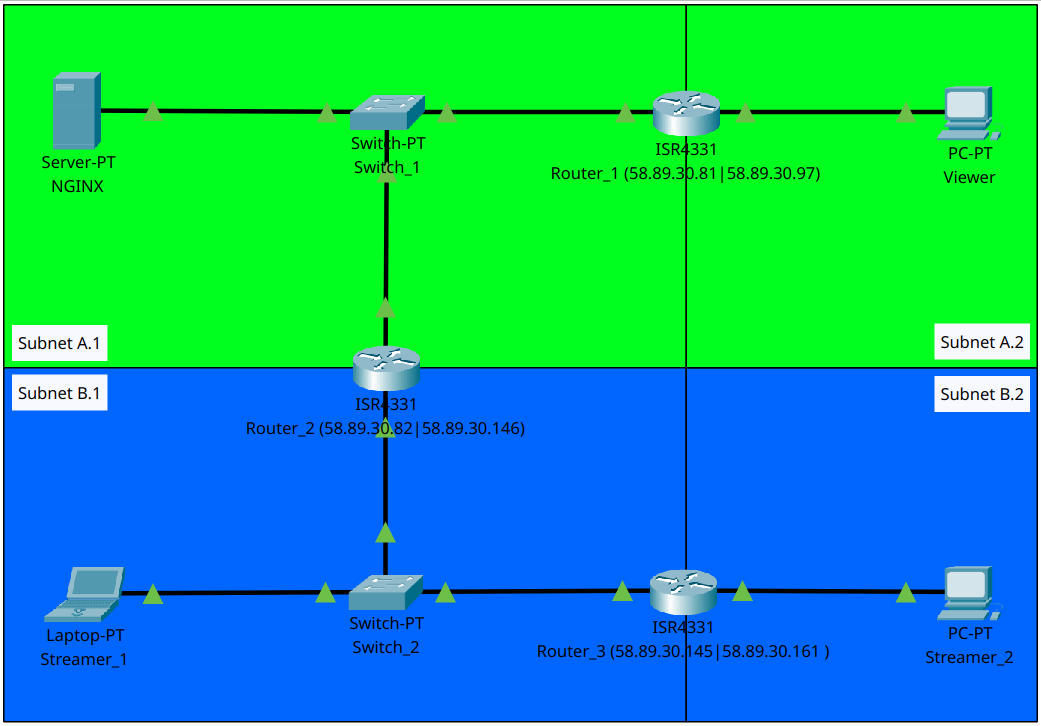
\includegraphics[width=\textwidth]{t.png}
	\caption{Our network made within \textit{Cisco Packet Tracer}.}
	\label{fig:topology}
\end{figure}
\pagebreak
\section{Roles}
Our group for project network consists of four students and we all had a role:
\begin{itemize}
	\item \textbf{Semih}:
	\begin{itemize}
		\item Router 2. Main role is the connectivity between subnet \textit{A} and \textit{B};
		\item Streamer 1.
	\end{itemize}
	\item \textbf{Ferhat}:
	\begin{itemize}
		\item Router 3. Main role is the connectivity between subnet \textit{B.1} and \textit{B.2}. Router 3 is also a DHCP-server;
		\item Streamer 2.
	\end{itemize}
	\item \textbf{Marvin}:
	\begin{itemize}
		\item Nginx. This server is going to receive the media stream from the Raspberry Pi, decrypt it, authenticate and serve it as both HLS and Dash.
	\end{itemize}
	\item \textbf{Thom}:
	\begin{itemize}
		\item Router 1. Main role is the connectivity between subnet \textit{A.1} and \textit{A.2}. Router 3 is also a DNS-server and DHCP-server;
		\item Viewer.
	\end{itemize} 
\end{itemize}
\pagebreak
\section{Streaming}
My role is to be both \textit{Router\_2} and \textit{Streamer\_1} in subnet B.1 as seen in \autoref{fig:topology}. \textit{Router\_2} has IPv4-forwarding enabled to act as a router. 

\subsection{Configuring IPv4-static routes}
Adding an IP-route is important for connectivity between all the devices. 
This is done with the following Linux command: ``\textit{sudo ip route add (IP-1) via (IP-2)}''. 
\textit{IP-1} and \textit{IP-2} are both variable IPv4-addresses.  
There was also a static route added for \textit{Router\_1} to redirect any packages going from:
\begin{itemize}
  \item 58.89.30.128/26 \textit{(subnet A)} via 58.89.30.82 \textit{(router\_2)} with subnet mask 255.255.255.192.
\end{itemize} 
There were also two static routes added for \textit{Router\_2} to redirect any packages going from:
\begin{itemize}
  \item 58.89.30.96/28 \textit{(subnet A.2)} via 58.89.30.81 \textit{(subnet A.1)} with subnet mask 255.255.255.240;
  \item 58.89.30.160/28 \textit{(subnet B.2)} via 58.89.30.145 \textit{(subnet B.1)} with subnet mask 255.255.255.240.
\end{itemize} 
There was also a static route added for \textit{Router\_3} to redirect any packages going from:
\begin{itemize}
  \item 58.89.30.64/26 \textit{(subnet B)} via 58.89.30.146 \textit{(router\_2)} with subnet mask 255.255.255.192.
\end{itemize} 
After configuring the routers properly, \autoref{fig:ping1} and \autoref{fig:ping2} confirm that I (as \textit{Router\_2}) was able to ping every device in both subnet A and B.
\subsection{FFmpeg streaming}
In order to stream something, \textit{streamer\_1} and \textit{streamer\_2} had to install a program called \textit{FFmpeg}. 
FFmpeg is a great tool to compress, convert, edit videos and images. 
It can also be used to stream a webcam or desktop environment. 
In order to stream my webcam, I entered the following command (for both \textit{streamer\_1} and \textit{streamer\_2}):

\begin{Verbatim}[frame=single, tabsize=4]
  ffmpeg -f v4l2 -i /dev/video0 \
    -c:v libx264 -pix_fmt yuv420p -framerate 15 -g 30 -b:v 500k \
    -preset ultrafast -tune zerolatency \
    -f flv "rtmp://58.89.30.83:4000/live/cam1?streamkey=123"
  \end{Verbatim}
  
In this command above, 
we captured the video source from the webcam using Video4Linux, compresses it and streams it to the RTMP-server, which in this case is: \textit{Nginx} (58.89.30.83) in subnet A.1 seen in \autoref{fig:topology}. 
It is also possible to stream my desktop environment by using \textit{x11grab} as shown in the following command below:
  
  \begin{Verbatim}[frame=single, tabsize=4]
  ffmpeg -video_size 1920x1080 -framerate 30 -f x11grab -i :0.0 \
    -c:v libx264 -pix_fmt yuv420p -framerate 15 -g 30 -b:v 500k \
    -preset ultrafast -tune zerolatency \
    -f flv "rtmp://58.89.30.83:4000/live/cam1?streamkey=123"
  \end{Verbatim}
Both commands worked on \textit{streamer\_1} as well for \textit{streamer\_2}. The viewer was able to connect to the RTMP-server and fetch the stream successfully! 
It does work as shown in \autoref{fig:samsho2}, \autoref{fig:mslug2}, \autoref{fig:webcam} and \autoref{fig:webcam2}, unfortunately there is a lot of latency. 
In the real world however, this won't matter as much because the streamer and viewer won't be sitting in the same room anyway. So latency would not be noticed that rapidly.
\pagebreak

\begin{figure}[H]
	\centering
	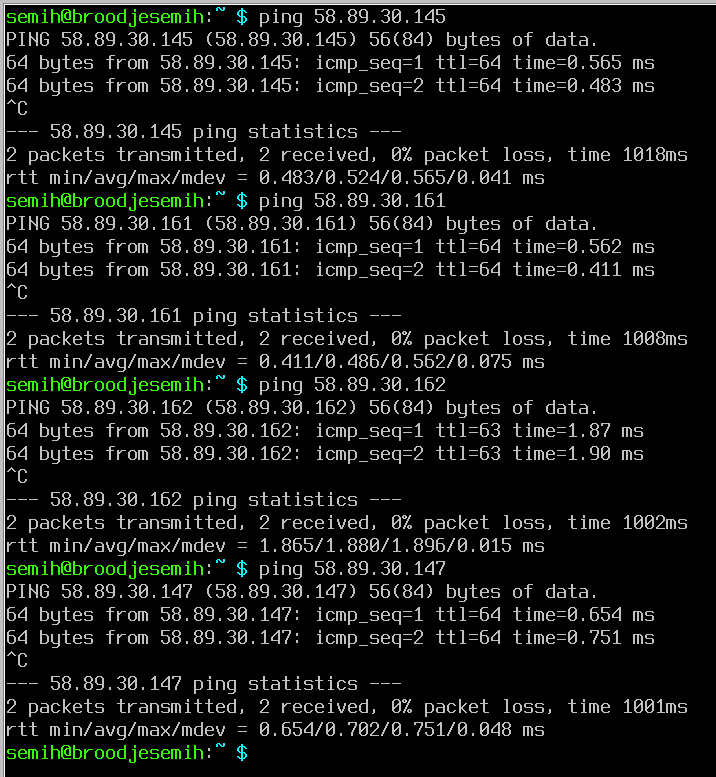
\includegraphics[width=13.5cm]{bewijs1.png}
	\caption{It's possible to ping every device on the network (pt.1).}
	\label{fig:ping1}
\end{figure}

\begin{figure}[H]
	\centering
	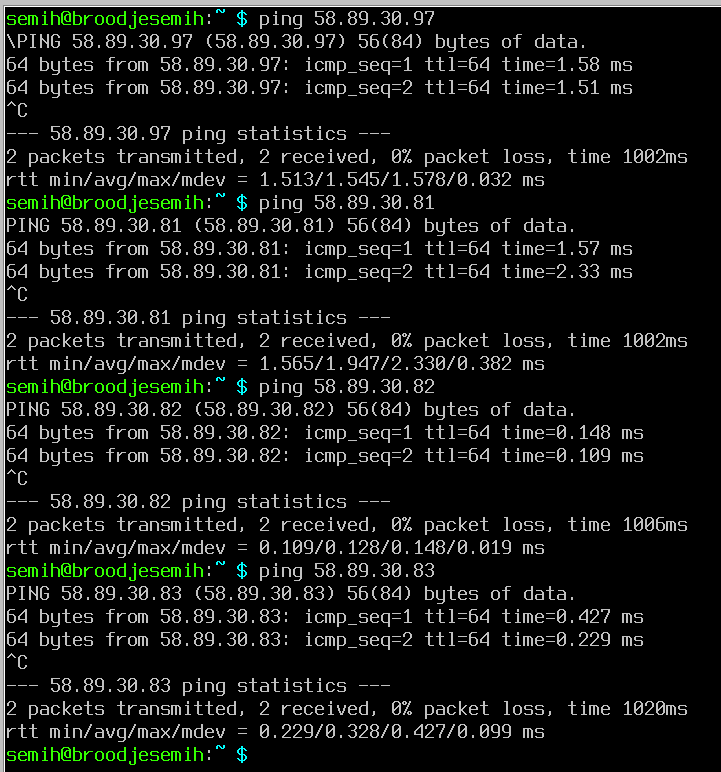
\includegraphics[width=13.5cm]{bewijs2.png}
	\caption{It's possible to ping every device on the network (pt.2).}
	\label{fig:ping2}
\end{figure}

\begin{figure}[H]
	\centering
	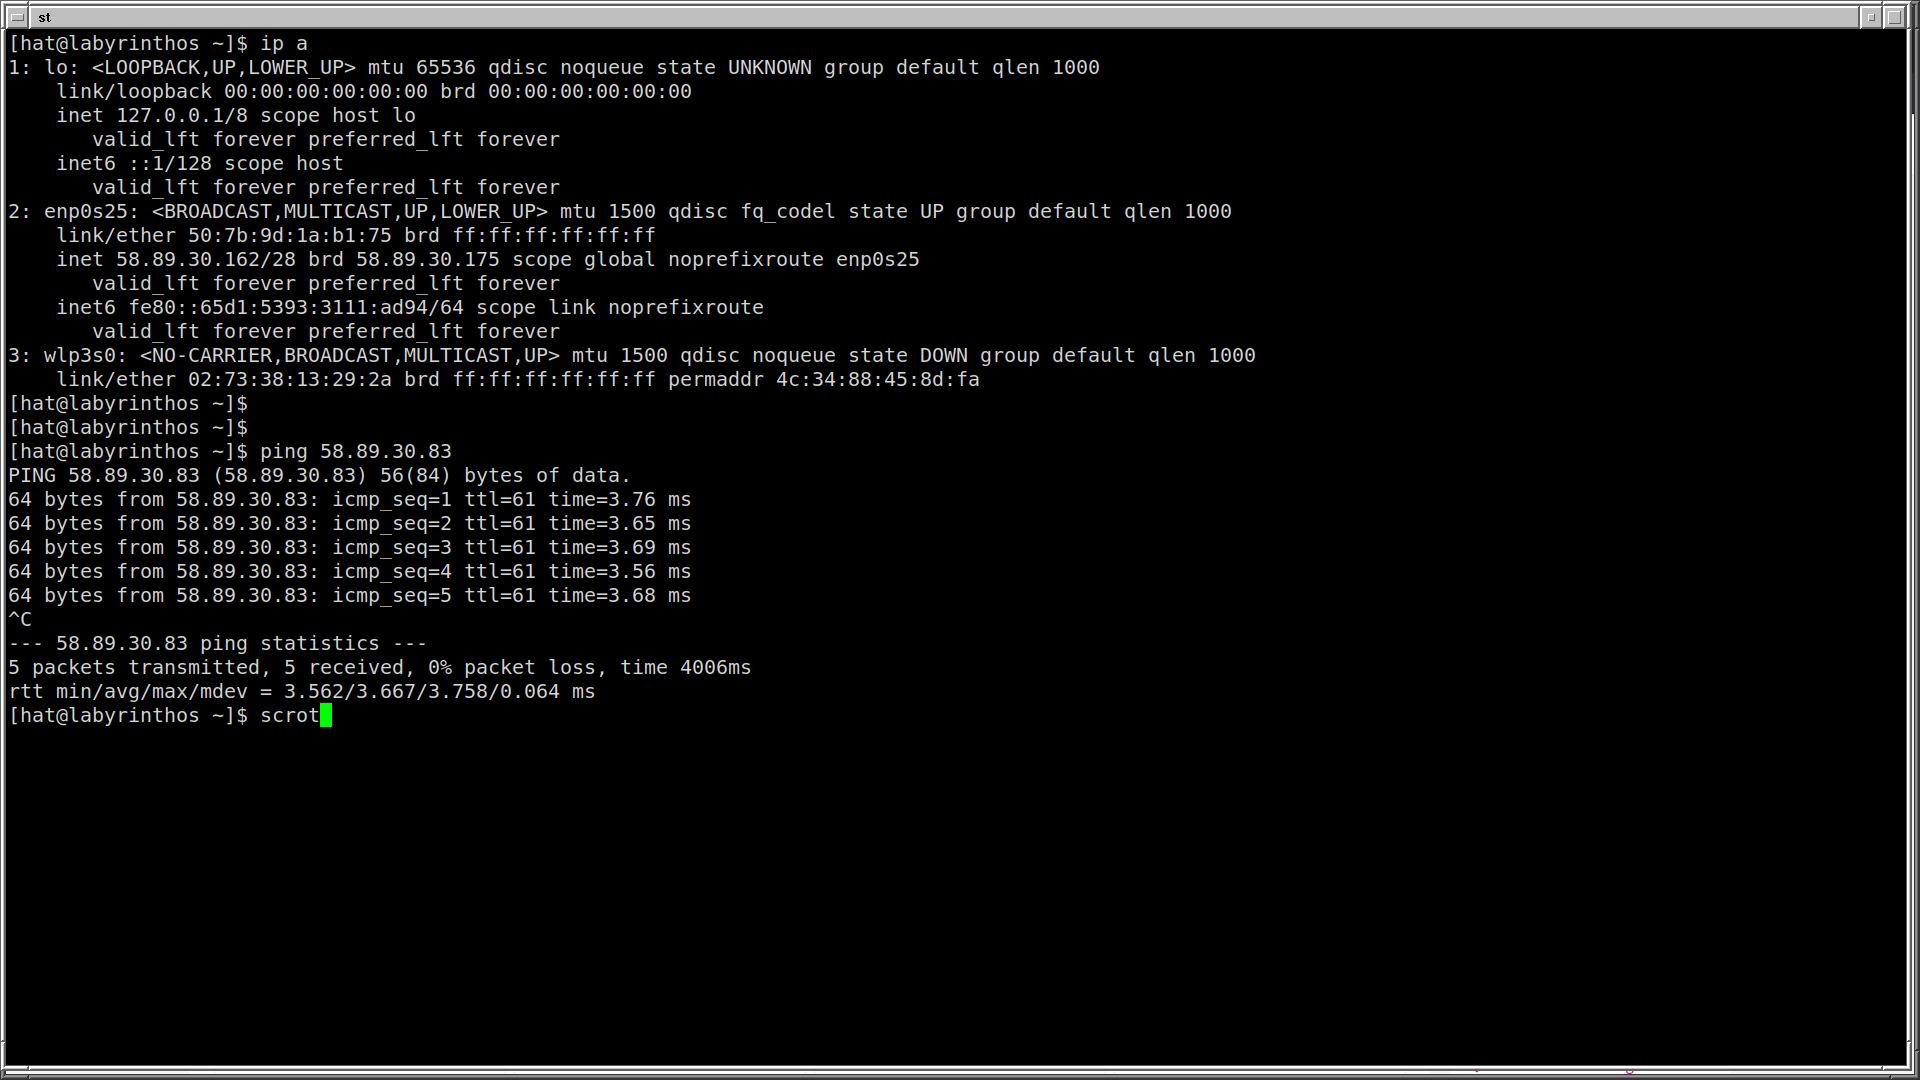
\includegraphics[width=13.5cm]{ping.png}
	\caption{It's possible to ping from subnet B to A.}
	\label{fig:ping}
\end{figure}

\begin{figure}[H]
	\centering
	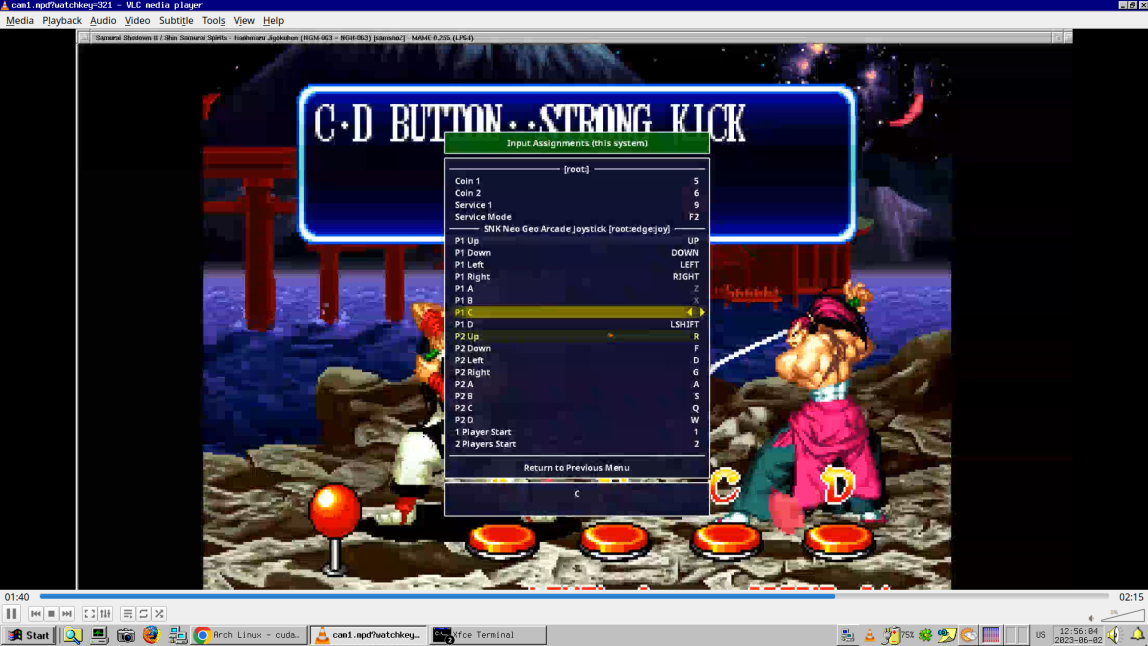
\includegraphics[width=\textwidth]{samsho2.png}
	\caption{Viewer watching gameplay of Samurai Shodown II (\textit{streamer\_2}). Note that the compression artifacts does make the image quite smeary.}
	\label{fig:samsho2}
\end{figure}

\begin{figure}[H]
	\centering
	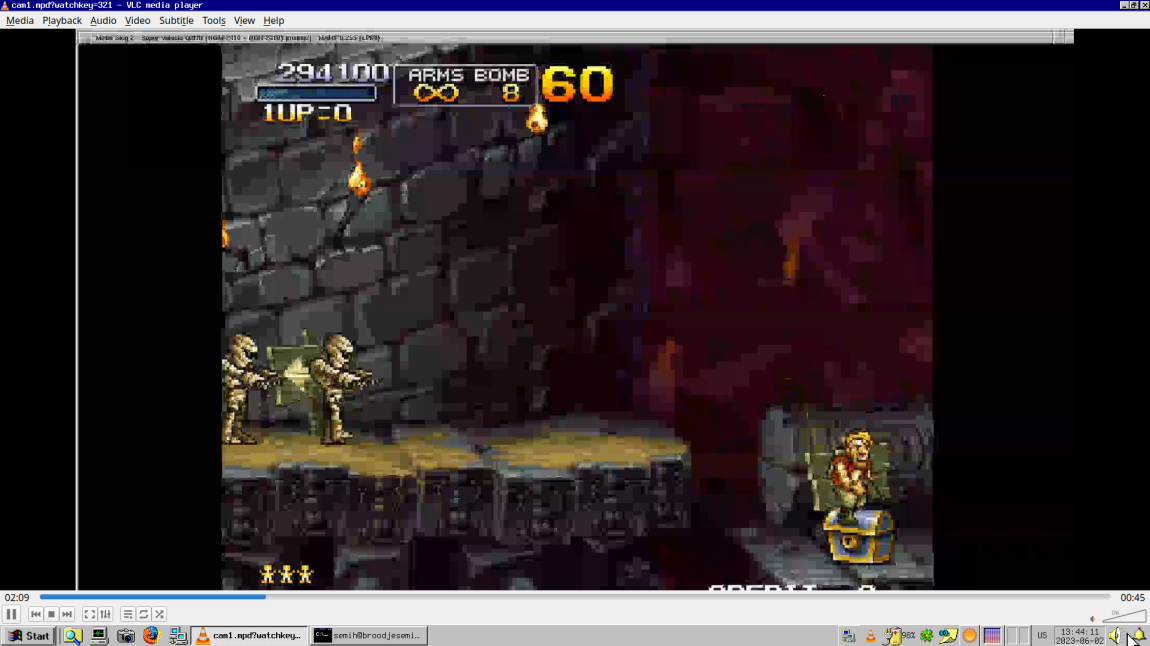
\includegraphics[width=\textwidth]{mslug2.png}
	\caption{Viewer watching gameplay of Metal Slug 2 (\textit{streamer\_2}). The compression artifacts is even worse on this one.}
	\label{fig:mslug2}
\end{figure}

\begin{figure}[H]
	\centering
	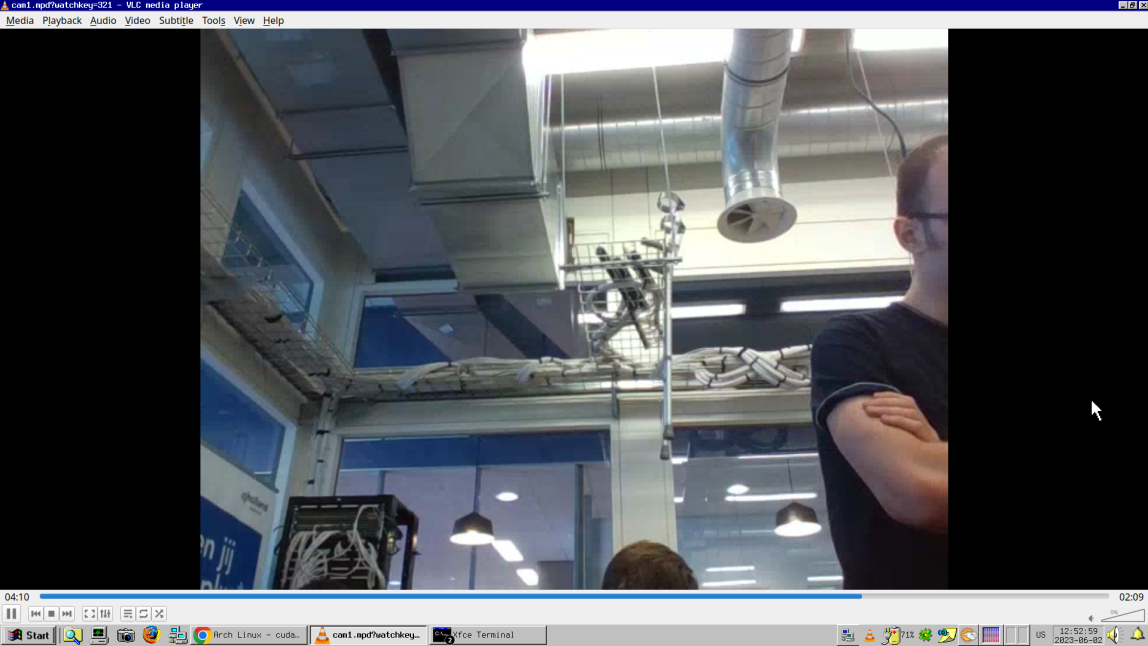
\includegraphics[width=\textwidth]{webcam.png}
	\caption{Viewer watching webcam of \textit{streamer\_2}.}
	\label{fig:webcam}
\end{figure}

\begin{figure}[H]
	\centering
	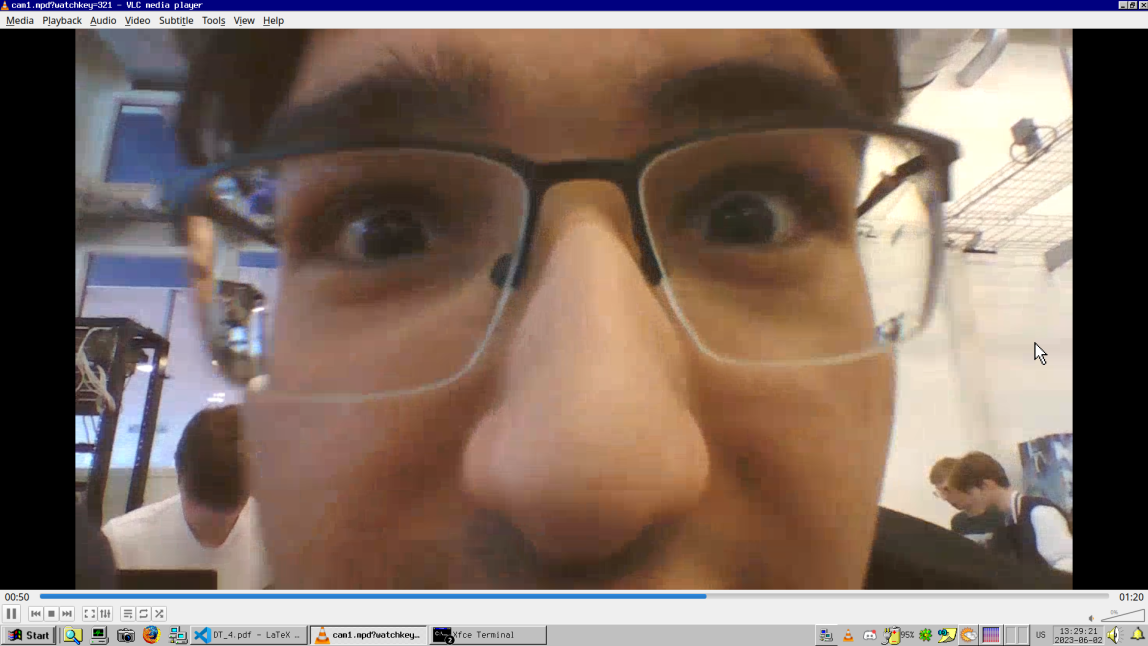
\includegraphics[width=\textwidth]{hello.png}
	\caption{\textit{streamer\_1} streaming and watching his own webcam.}
	\label{fig:webcam2}
\end{figure}


\section{Miscellaneous screenshots}
\begin{figure}[H]
	\centering
	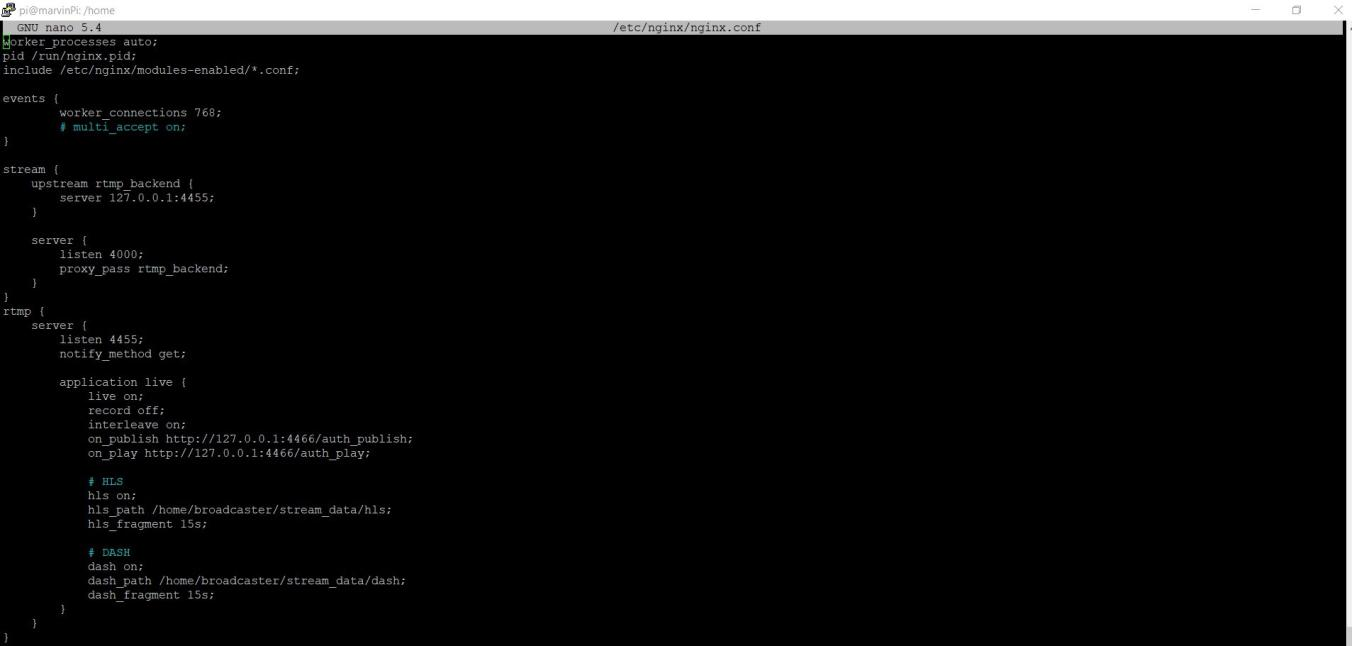
\includegraphics[width=\textwidth]{n1.jpg}
	\caption{Nginx configuration for RMTP-server, which all has been done by Marvin (pt.1).}
	\label{fig:n1}
\end{figure}

\begin{figure}[H]
	\centering
	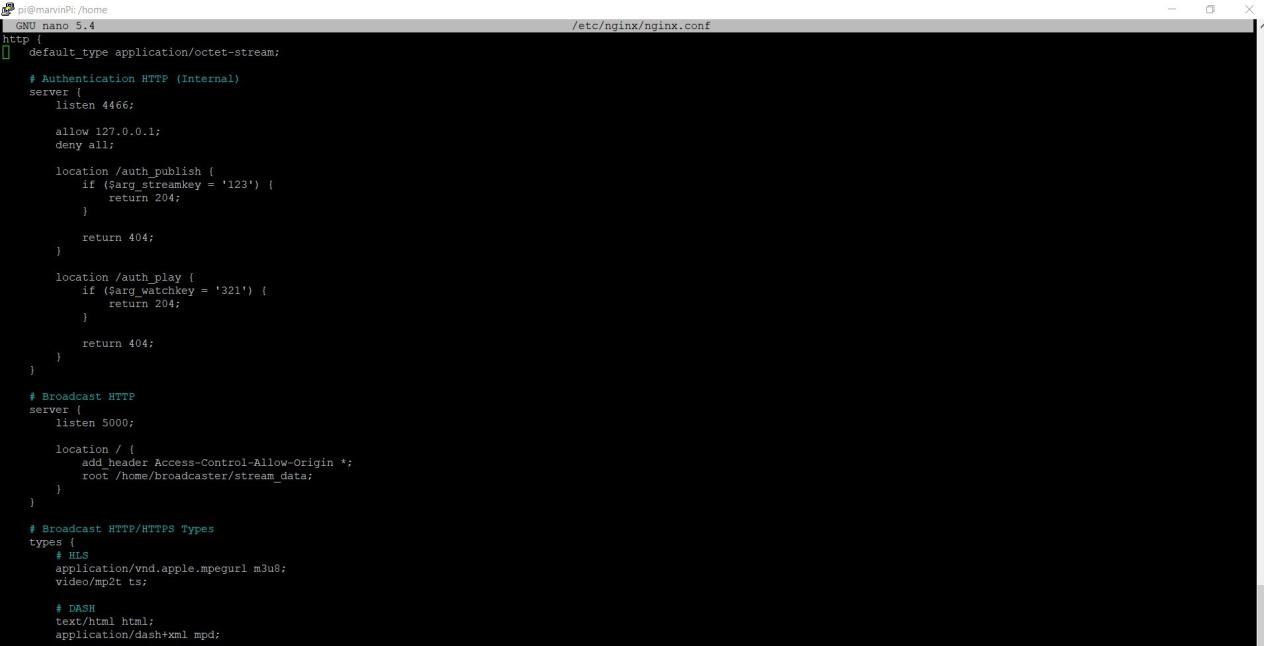
\includegraphics[width=\textwidth]{n2.jpg}
	\caption{Nginx configuration for RMTP-server, which all has been done by Marvin (pt.2).}
	\label{fig:n2}
\end{figure}

\begin{figure}[H]
	\centering
	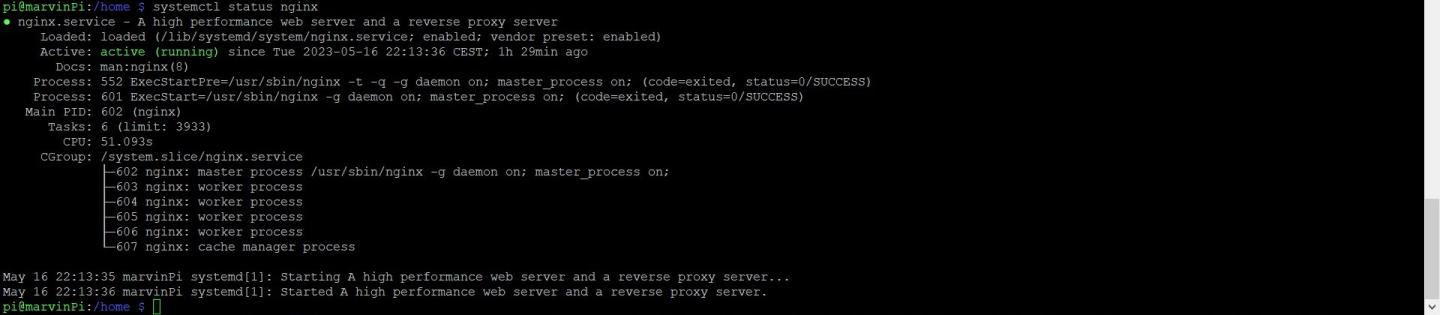
\includegraphics[width=\textwidth]{n3.jpg}
	\caption{Proof of that the Nginx-server is running without any problems!}
	\label{fig:n3}
\end{figure}

\begin{figure}[H]
	\centering
	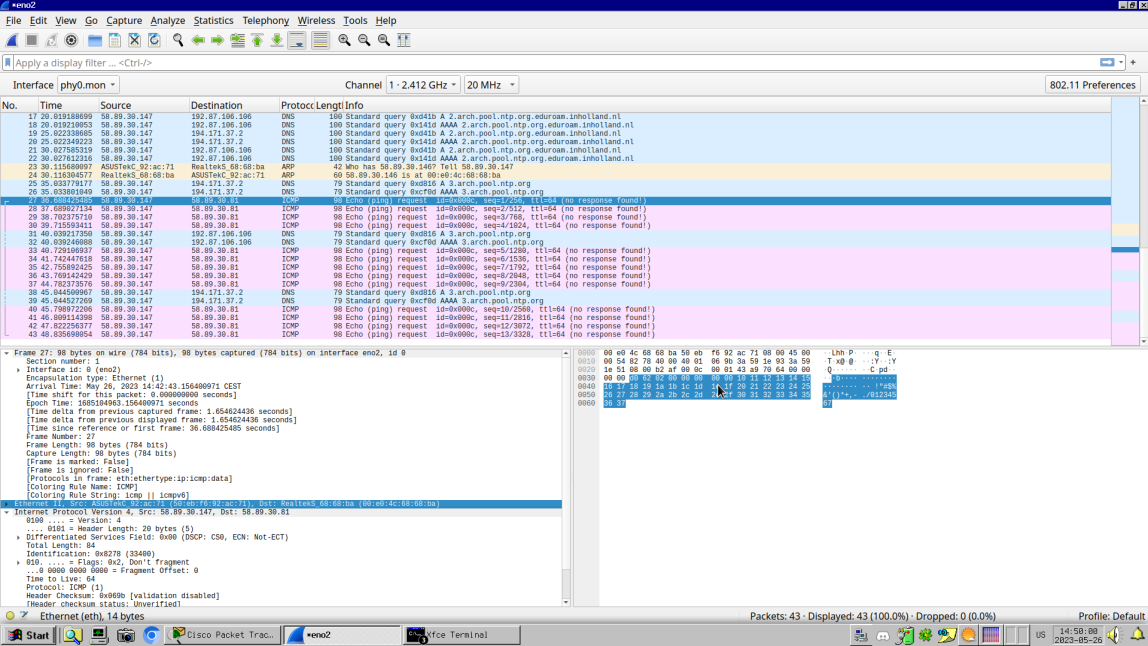
\includegraphics[width=\textwidth]{ws.png}
	\caption{Here was I (Semih) troubleshooting the ICMP (ping) request via my laptop (58.89.30.147) to \textit{router\_1} (58.89.30.81).}
	\label{fig:ws}
\end{figure}

\begin{figure}[H]
	\centering
	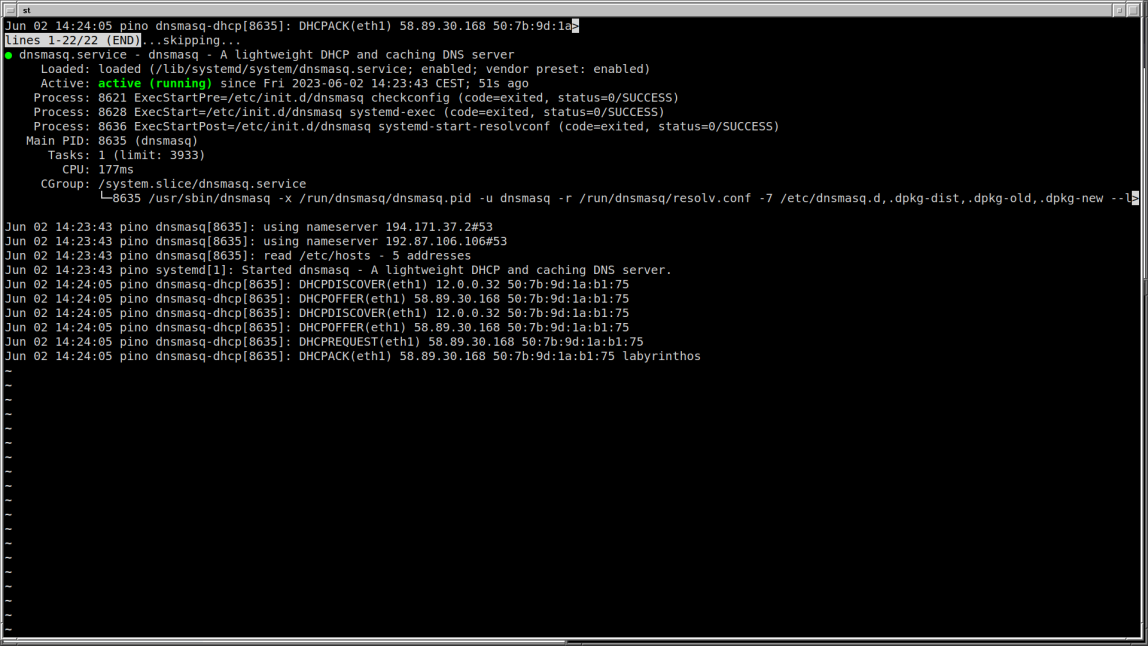
\includegraphics[width=\textwidth]{dhcp.png}
	\caption{DHCP-server is working fine in subnet B.2 (\textit{router\_3}).}
	\label{fig:dhcp}
\end{figure}

\begin{figure}[H]
	\centering
	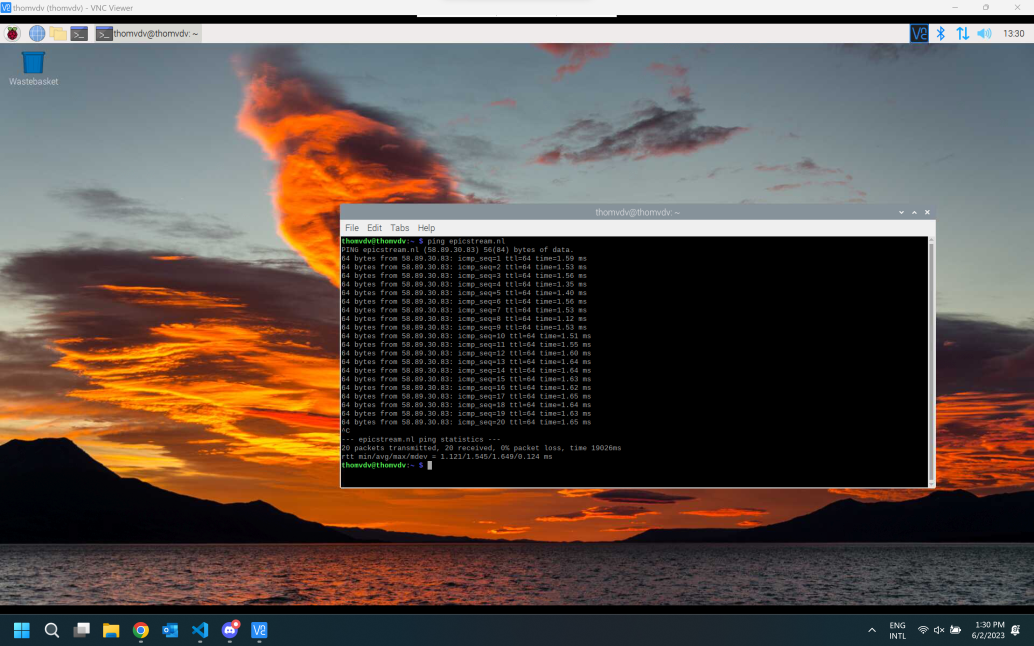
\includegraphics[width=\textwidth]{dns.png}
	\caption{DNS-server is working fine in subnet A.1 \textit{router\_1}.}
	\label{fig:dns}
\end{figure}

\begin{figure}[H]
	\centering
	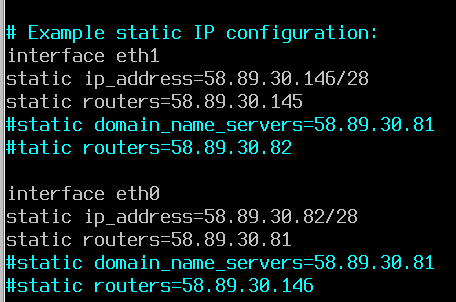
\includegraphics[width=\textwidth]{config1.png}
	\caption{dhcpcd.conf file of \textit{router\_2}.}
	\label{fig:dhcpcd}
\end{figure}

\begin{figure}[H]
	\centering
	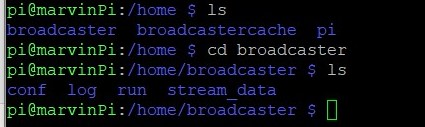
\includegraphics[width=\textwidth]{FoldersNGINX.jpg}
	\caption{ls command in MarvinPi (\textit{Nginx}).}
	\label{fig:marvin}
\end{figure}

\begin{figure}[H]
	\centering
	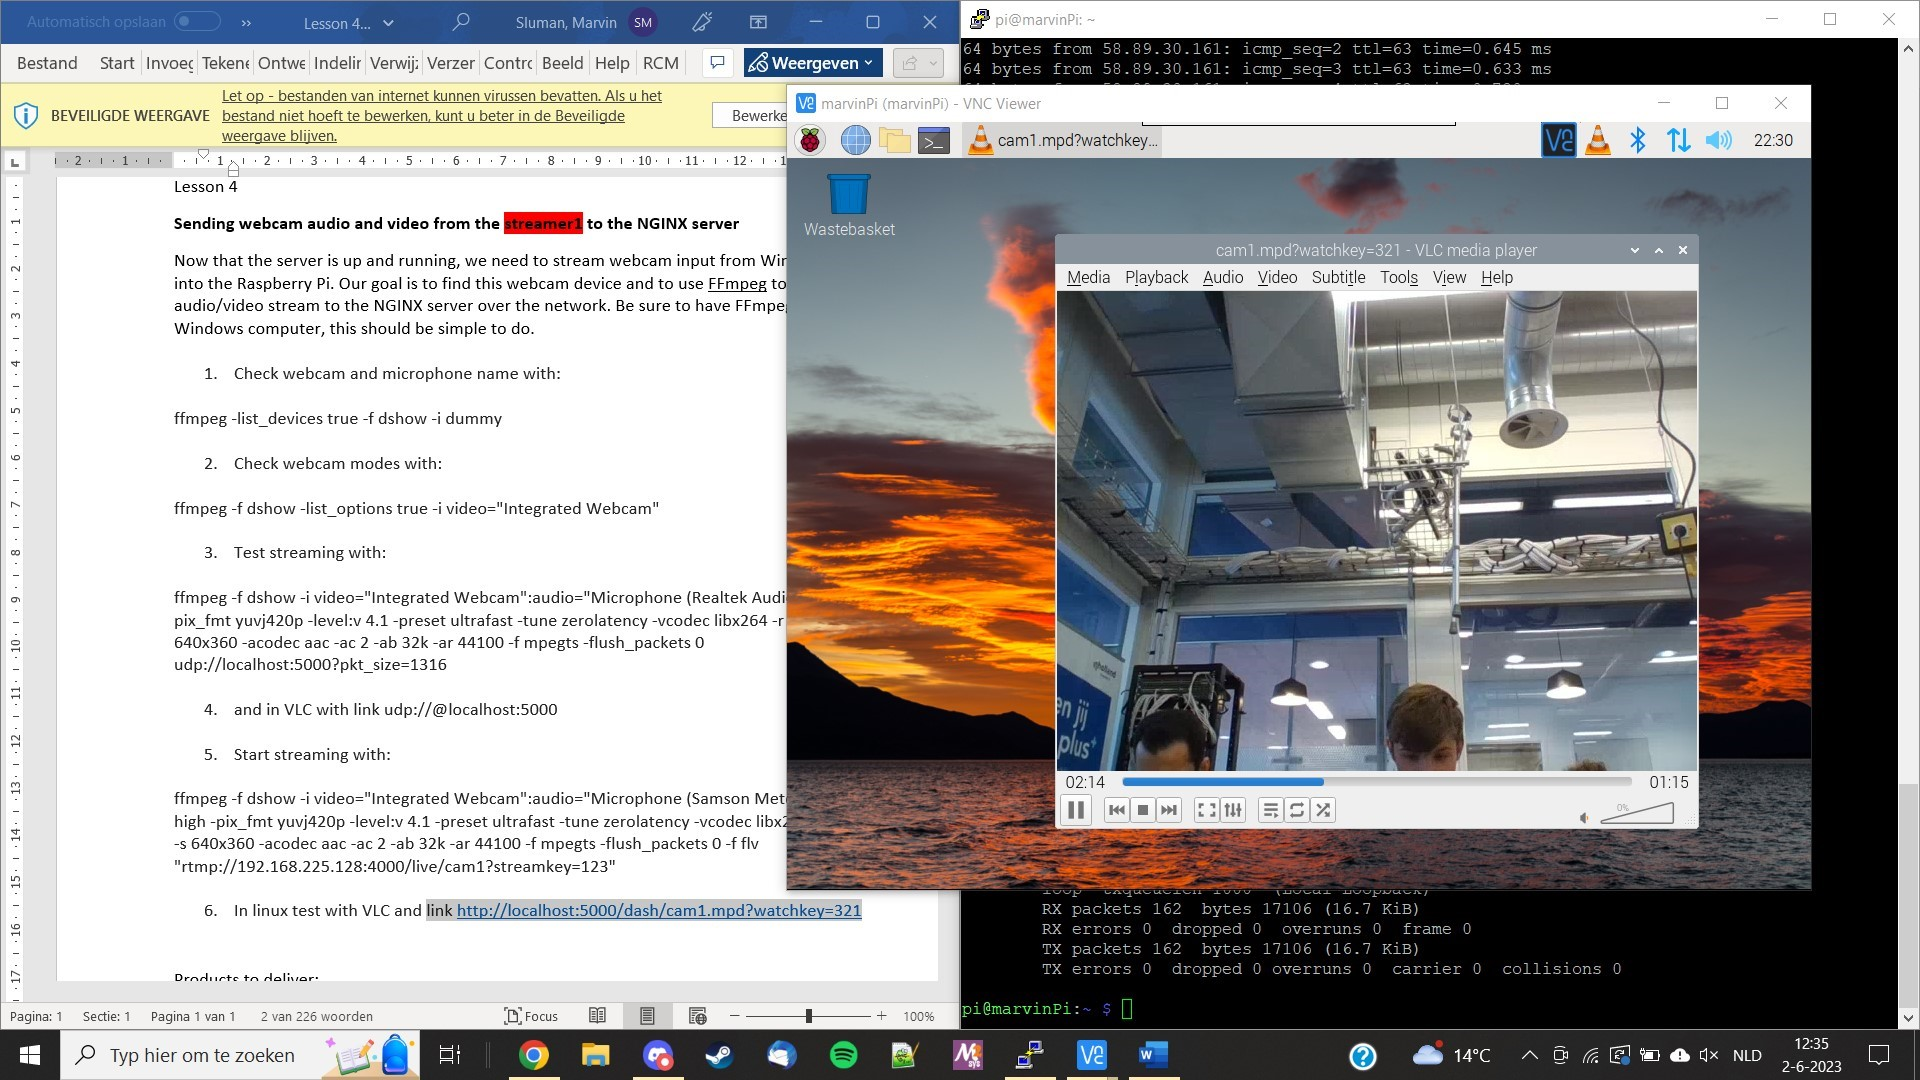
\includegraphics[width=\textwidth]{WorkingStream.jpg}
	\caption{Marvin watching \textit{streamer\_2} (via \textit{Nginx}).}
	\label{fig:marvi2n2}
\end{figure}

\begin{figure}[H]
	\centering
	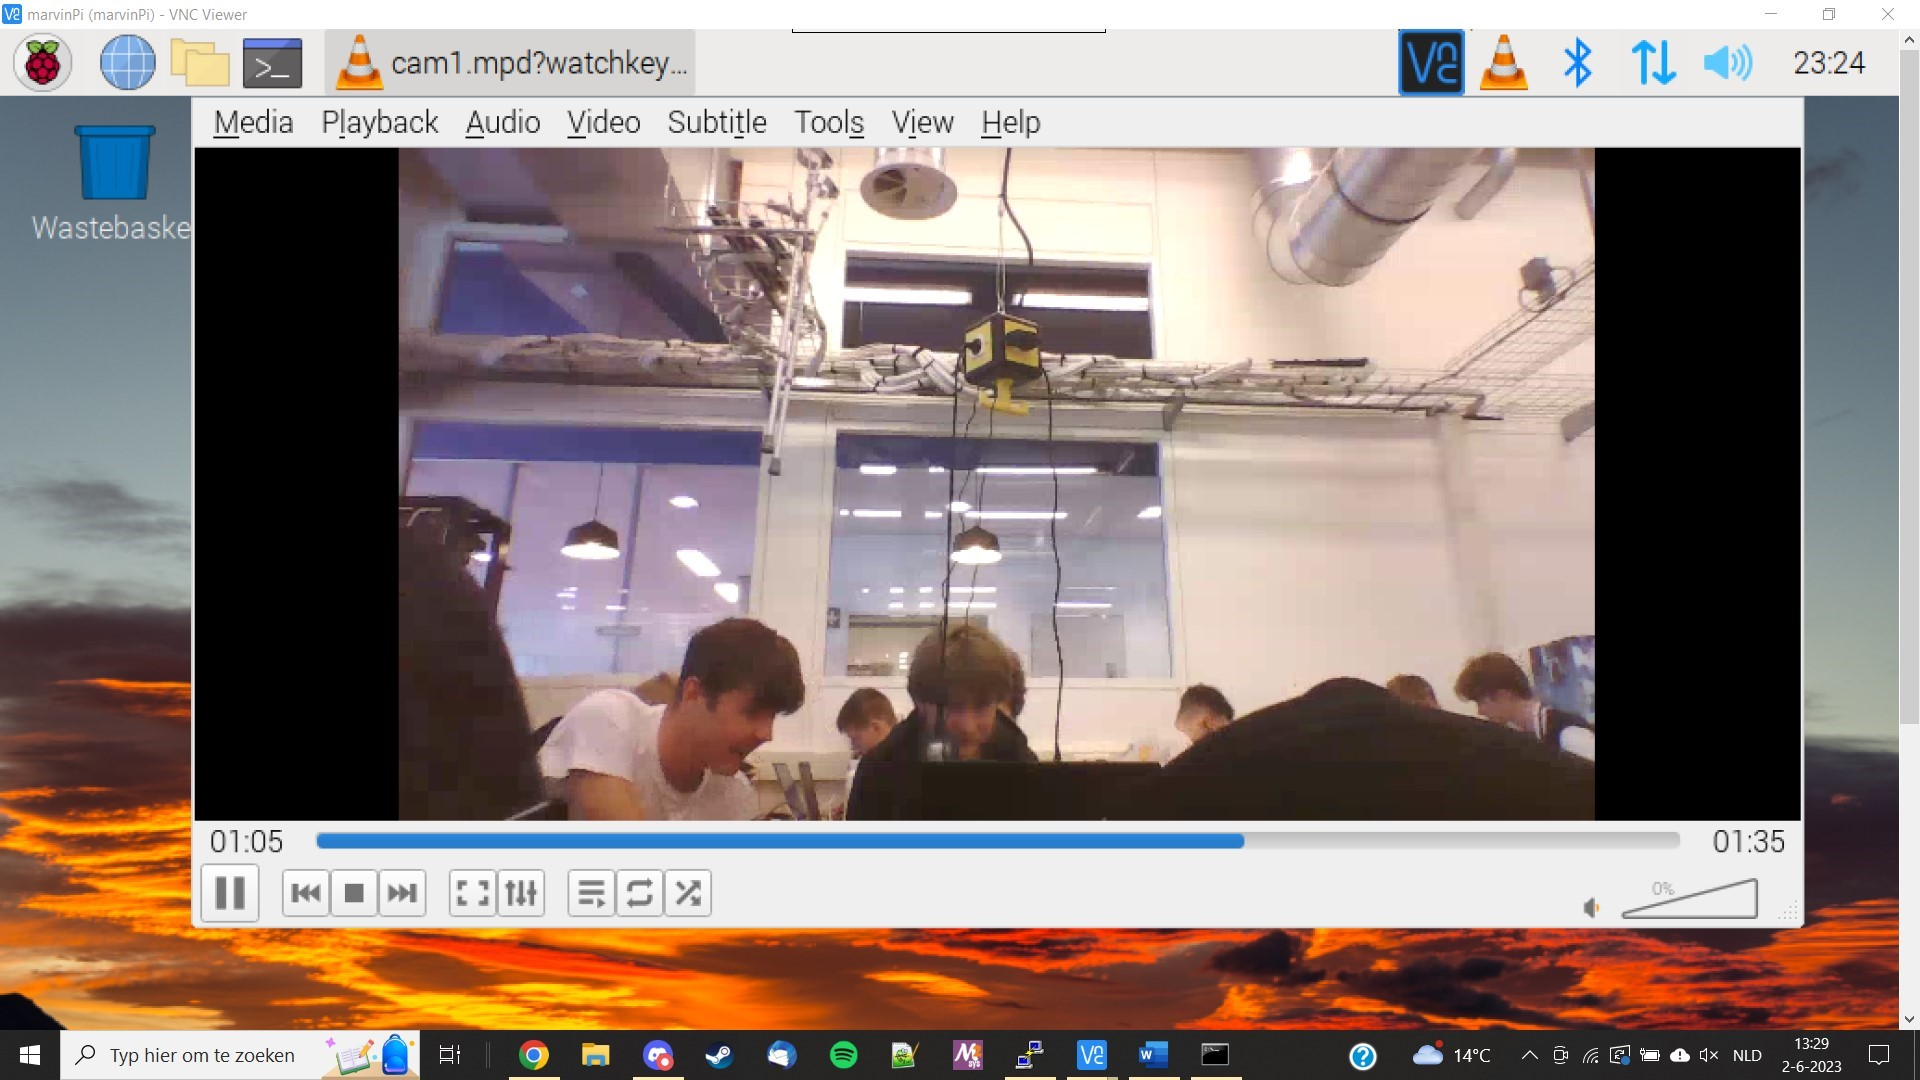
\includegraphics[width=\textwidth]{WorkingStream2.jpg}
	\caption{Marvin watching \textit{streamer\_1} (via \textit{Nginx}).}
	\label{fig:mar2vi2n2}
\end{figure}

\begin{figure}[H]
	\centering
	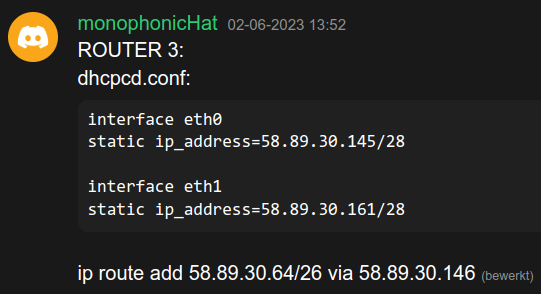
\includegraphics[width=\textwidth]{ferhat.png}
	\caption{\textit{Router\_3 } dhcpcd.conf file.}
	\label{fig:ferhat2}
\end{figure}

\begin{figure}[H]
	\centering
	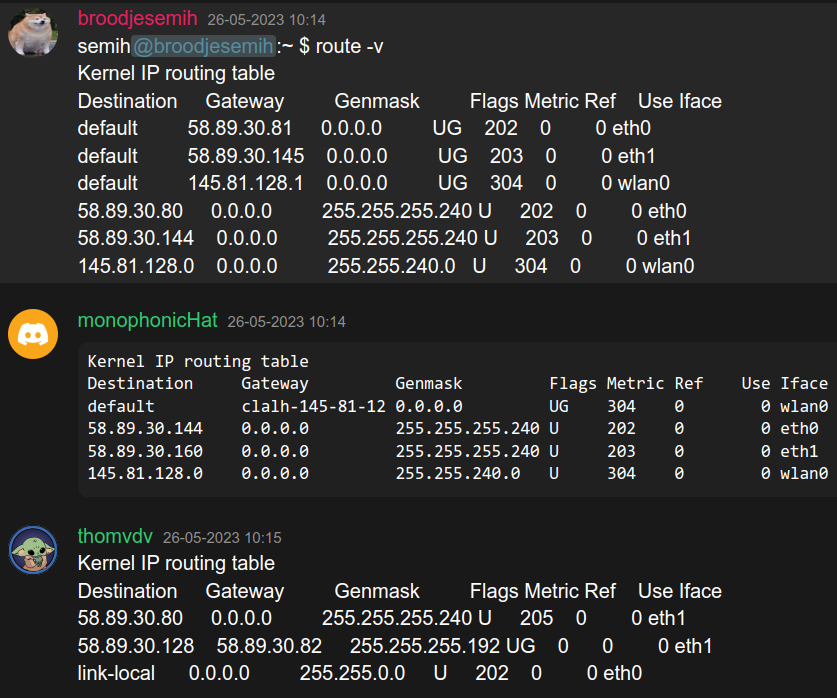
\includegraphics[width=\textwidth]{routetable.png}
	\caption{All ``route -v'' outputs.}
	\label{fig:ferhsat2}
\end{figure}


\begin{figure}[H]
	\centering
	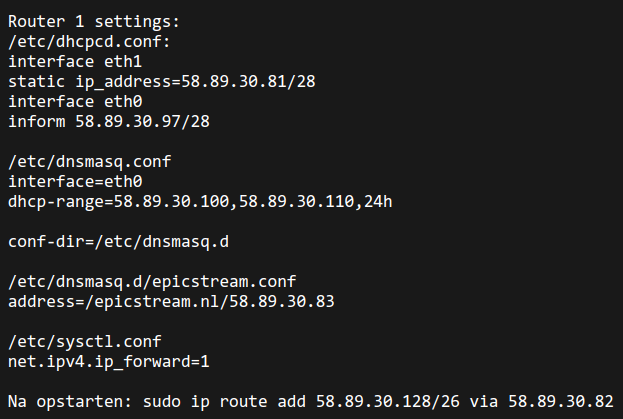
\includegraphics[width=\textwidth]{thomconf.png}
	\caption{\textit{Router\_1 } config files.}
	\label{fig:ssdsad}
\end{figure}


\pagebreak
\end{document}